\documentclass[12pt, oneside]{article}
\usepackage{geometry}
\usepackage[utf8]{inputenc}
\usepackage{setspace}
\usepackage{times}
\usepackage{url}
\urlstyle{same}
\usepackage{multirow}
\usepackage[usegeometry]{typearea}
% Useful for checking layout
% \usepackage{showframe}
\usepackage{fancyhdr}
\usepackage{blindtext}
% Indenting the first sentence after section
\usepackage{indentfirst}
% Set language
\usepackage[german]{babel}
% Abbreviations
\usepackage{glossaries}
% For big tables which span multiple pages
\usepackage{longtable}
% Images
\usepackage{graphicx}
\graphicspath{ {./images/} }
% APA Citation Style
\usepackage[natbibapa]{apacite}
% Smaller font size for captions
\usepackage[font=small,labelfont=bf]{caption}
% Table related packages
\usepackage{booktabs}


\geometry{
 a4paper,
 left=30mm,
 top=25mm,
 right=25mm,
 bottom=20mm,
 footskip=15pt,
}

\setstretch{1.3} % Define Line Spacing
\renewcommand{\headrulewidth}{0pt} % Remove footer line

\pagestyle{fancy} % Allow for customizing header and footer
% Customize footer for page number location
\fancyhf{}
\fancyfoot{}
\fancyhead[R]{Yannick Hutter}
\fancyhead[L]{Bachelorthesis}
\fancyfoot[R]{\thepage}



 \makeglossaries

 \newglossaryentry{dsr}
 {
     name=DSR,
     description={Design science Research}
 }
 
 \newglossaryentry{covid19}
 {
     name=COVID-19,
     description={Coronavirus-Krankheit-2019 ~\citep{covid19}}
 }
 \newglossaryentry{bfs}
 {
     name=BFS,
     description={Bundesamt für Statistik}
 }
 
 \newglossaryentry{foph}
 {
     name=FOPH,
     description={Federal Office of Public Health}
 }
 \newglossaryentry{fhgr}
 {
     name=FHGR,
     description={Fachhochschule Graubünden}
 }
 \newglossaryentry{svi}
 {
     name=SVI,
     description={Social Vulnerability Index}
 }
 \newglossaryentry{who}
 {
     name=WHO,
     description={World Health Organisation}
 }



\begin{document}
\pagenumbering{roman}
\begin{titlepage}
	\begin{center}
		\Huge
		\textbf{Bachelorthesis}\\
		\vspace{0.5cm}
		\LARGE
		Analyse und Implementierung eines personalisierbaren Corona Dashboards für Millenials

		\vspace{1.5cm}
		\normalsize
		\textbf{Yannick Hutter}\\
		\textbf{Digital Business Management Klasse 18tz}\\
		\textbf{Talackerstrasse 8}\\
		\textbf{8887 Mels}\\
		\textbf{yannick.hutter@stud.fhgr.ch}\\


		\vfill
		Referrent: Daniel Klinkhammer\\
		Korefferent: Michael Burch\\

		\vspace{0.8cm}


		Digital Business Management\\
		Fachhochschule Graubünden\\
		Mels, April 2022
	\end{center}
\end{titlepage}

\clearpage
\section*{Abstract}
TODO


\clearpage
\tableofcontents

\clearpage
\listoffigures
\listoftables

\clearpage
\printglossaries

\pagenumbering{arabic}

\clearpage
\section{Einleitung}
Seit Beginn der Menschheitsgeschichte gab es bereits unzählige Pandemien, welche Ihren Tribut gefordert haben. Die neuste Pandemie, auch bekannt unter dem Namen \Gls{covid19}, ist hierbei keine Ausnahme und zählt zu den Spitzenreitern in Bezug auf die tägliche Anzahl krankheitsbedingter Todesfälle (siehe Abbildung 1).

\begin{figure}[ht]
    \includegraphics[width=12cm]{images/krankheitsbedingte_todesfälle_nach_erkrankung.png}
    \centering
    \caption{Durchschnittliche tägliche Anzahl krankheitsbedingter Todesfälle weltweit nach Erkrankung (Stand:
1. Januar 2021) ~\citep[S. 12]{worldwide_epidemic_cases_study}}
\end{figure}

\Gls{covid19}, fortlaufend als Corona bezeichnet, hat sowohl in den wirtschaftlichen als auch in den sozialen Strukturen tiefgreifende Veränderungen herbeigeführt. Um die Bevölkerung auf die Gefahr der Pandemie zu sensibilisieren und die rasant steigenden Fallzahlen (siehe Abbildung 2) des Virus einzudämmen, wurden diverse Anstrengungen unternommen.

\begin{figure}[ht]
    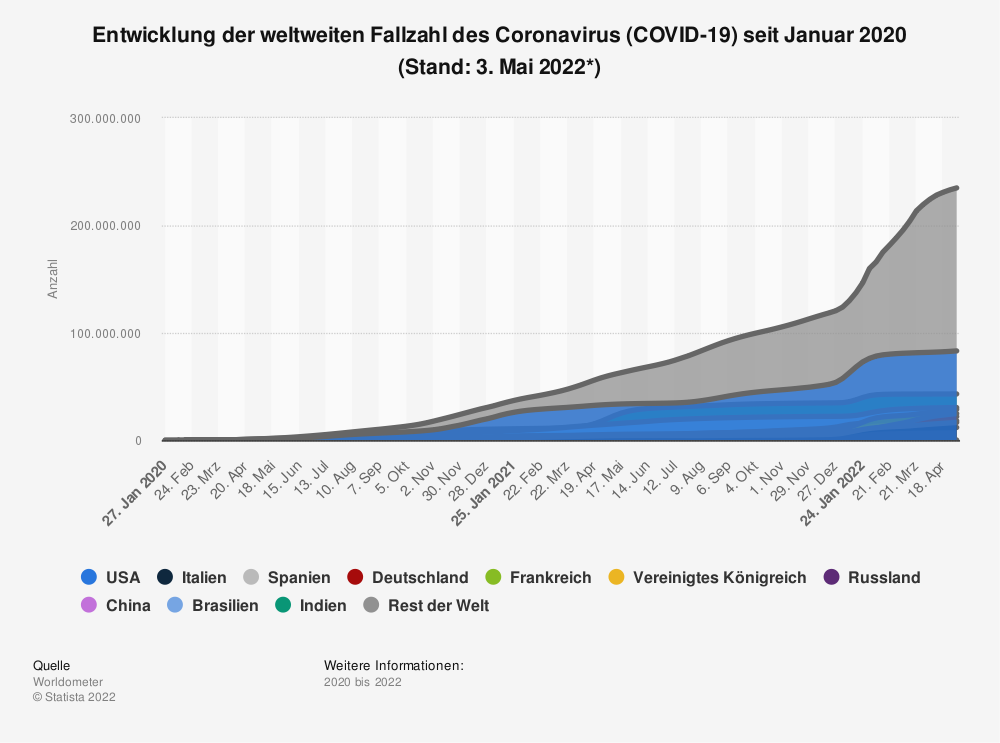
\includegraphics[width=10cm]{images/corona_fallzahlen.png}
    \centering
    \caption{Entwicklung der weltweiten Fallzahl des Coronavirus (COVID-19) seit Januar 2020 ~\citep{covid_cases_worldwide}}
\end{figure}

Eine zentrale Rolle spielten hierbei \textit{Datenvisualisierungen}. Wichtig in diesem Kontext zu verstehen, ist es, dass sich der Begriff Datenvisualisierungen nicht nur aus Linien- oder Kuchendiagrammen definiert, sondern ein breites Spektrum von verschiedenen Visualisierungsarten, darunter auch Infografiken, abdeckt. So erstellte zum Beispiel das \Gls{bfs} diverse Infografiken in den Bereichen Gesundheit, Kultur sowie Kriminalität, in Bezug auf Corona ~\citep{covid19_bfs_infografiken}.

Besonders während einer weltweiten Pandemie wie Corona ist eine akkumulierte Sicht von verschiedenen Visualisierungsarten von zentraler Bedeutung. Dies kann mit Hilfe von \textit{Dashboards} bewerkstelligt werden. Der Begriff Dashboard kommt ursprünglich aus dem Englischen und bezieht sich auf das Armaturenbrett des Autos, wo alle relevanten Informationen übersichtlich auf einem Blick sichtbar sind ~\citep{Duden.18.04.2022}. In Bezug auf Corona werden auf Dashboards unter anderem wichtige Informationen wie Ansteckungszahlen und Todesfälle visualisiert. Ein Beispiel für ein Dashboard ist das \textit{WHO Coronavirus Dashboard}, welches von der \Gls{who} erstellt wurde ~\citep{who_dashboard}. Dass nebst dem in der Schweiz angesiedelten BFS selbst eine weltweite Organisation wie WHO sich um die Erstellung von Dashboards zur Corona Thematik bemüht, soll aufzeigen wie wichtig Datenvisualisierungen und insbesondere Dashboards geworden sind.

\subsection{Stand der Forschung}
Die Coronavirus-Pandemie greift seit ihrem Aufkommen im Jahr 2019 in eine Vielzahl von Lebensbereichen ein. Es ist wenig verwunderlich, dass zu einem solch einschnei-dendem Thema eine grosse Anzahl von wissenschaftlichen Publikationen erstellt worden sind. Eine Publikation untersuchte die Vielzahl von Corona Datenvisualisierungen und weist ihnen verschiedene Arten von Intentionen (Aussage über den Verlauf der Pandemie etc.) zu ~\citep{YixuanZhang.}. Weitere Quellen untersuchten speziell für das Web zugeschnittene Corona Dashboards und leiteten daraus Design Guidelines ab ~\citep{Ivankovic.2021}. Andere Studien wiederum haben sich mit der Erstellung von Dashboards für spezielle Nutzergruppen auseinandergesetzt ~\citep{Ivanov.2018}. Auch wurde bereits im Zuge einer Studie die Schwierigkeiten bei der Erstellung von Corona Dashboards aus dem Blickwinkel der eigentlichen Ersteller evaluiert ~\citep{Barbazza.}. Jedoch scheint es zum jetzigen Zeitpunkt noch keine Studie zu geben, welche die Erstellung von \textbf{personalisierbaren} Corona Dashboards für eine bestimmte Zielgruppe behandelt unter Berücksichtigung eines Nutzerzentrierten Vorgehens untersucht.


\subsection{Forschungsfrage}
Die Landschaft der Corona Datenvisualisierungen ist sehr breit gestrickt und umfasst unterschiedlichste Repräsentanten von Visualisierungsarten. Nebst den einzelnen Visualisierungen wie Liniendiagramme, welche den zeitlichen Verlauf von einzelnen Variablen (z.Bsp Corona Ansteckungszahlen) aufzeigen, werden diese aber auch in Form von Dashboards zusammengefasst. Eine grosse Anzahl dieser Dashboards sind jedoch  allgemein gehalten und fokussieren sich auf die breite Öffentlichkeit oder Datenanalysten. Auch gibt es von der Nutzerseite her \textbf{wenig Personalisierungsmöglichkeiten}. Anpassungen an bereits erstellten Dashboards sind in der Regel nicht vorgesehen. Interessant in diesem Kontext ist es zu untersuchen, wie sich eine spezifische Nutzergruppe ein personalisierbares Corona Dashboard vorstellt und welche \textbf{Visualisierungsarten} von Relevanz sind. Aufgrund dieser explorativen Fragestellung ergibt sich folgende übergeordnete Forschungsfrage:


\begin{center}
\textbf{Wie stellen sich Millennials ein personalisierbares Corona Dashboard vor?}
\end{center}

Um diese Forschungsfrage abzudecken, wurden folgende untergeordnete Fragestellungen formuliert:

\begin{center}
\textbf{Welche Visualisierungstypen in Bezug auf Corona werden von Millennials im Kontext eines personalisierbaren Corona Dashboards gefordert?\\
(untergeordnete Forschungsfrage 1)}
\end{center}

\begin{center}
\textbf{Welche Informationen in Bezug auf Corona werden von Millennials für ein Corona Dashboard gefordert?\\
(untergeordnete Forschungsfrage 2)}
\end{center}

\begin{center}
\textbf{Welche Personalisierungsmöglichkeiten werden von Millennials in Bezug auf Corona Dashboards gefordert?\\
(untergeordnete Forschungsfrage 3)}
\end{center}

\subsection{Methodische Vorgehensweise}
TODO

\clearpage
\section{Problemidentifizierung und Motivation}
TODO

\subsection{Dashboard – Ein Begriff mit Ursprung in der Automobilindustrie}
TODO

\subsection{Die wichtigsten Komponenten und Typen von Dashboards}
TODO

\subsection{Überblick über die bestehenden Corona Dashboards}
TODO

\subsection{Motivation – Erstellung eines personalisierbaren Corona Dashboards für Millennials}
TODO

\clearpage
\section{Identifikation der Ziele}
TODO

\subsection{Erstellung des Untersuchungsinstrumentes}
TODO

\subsection{Evaluation von Visualisierungstypen für Corona Dashboards}
TODO

\subsection{Identifikation von relevanten Personalisierungsmöglichkeiten in Bezug auf Dashboards}
TODO

\clearpage
\section{Design und Development}
TODO

\subsection{Design mittels Sketching}
TODO

\subsection{High-Fidelity Prototyp als Web Applikation}
TODO

\clearpage
\section{Auswertung}
TODO

\clearpage
\section{Fazit}
TODO

\clearpage
\section{Reflexion und Limitationen}
TODO


\clearpage
\bibliographystyle{apacite}
\urlstyle{rm}
\bibliography{main.bib}

\clearpage
\section*{Anhang}
\begin{table}[ht]
	\begin{tabular}{@{}p{4cm}p{4cm}p{6.5cm}@{}}
		\toprule
		\textbf{Quelle} & \textbf{Schlüsselwörter}        & \textbf{Artikel}        \\ \midrule
		\url{https:                                                                 \\scholar.google.com}                         & covid dashboard                 & ~\citep{Dong.2020}         \\ \midrule
		                &                                 & ~\citep{Florez.2020}    \\ \midrule
		                &                                 & ~\citep{Berry.2020}     \\ \midrule
		                & user centered dashboards        & ~\citep{Francois.2021}  \\ \midrule
		                &                                 & ~\citep{Young.2020}     \\ \midrule
		                & customizable dasbhoards         & ~\citep{Roberts.2017}   \\ \midrule
		\url{https:                                                                 \\dl-acm.org}                                 & covid19 dashboard               & ~\citep{Vitale.}           \\ \midrule
		                & evaluating crisis dashboards    & ~\citep{Ivanov.2018}    \\ \midrule
		                & data dashboards                 & ~\citep{Maheshwari.}    \\ \midrule
		                &                                 & ~\citep{Beheshti.}      \\ \midrule
		\url{https:                                                                 \\google.com}                                 & covid dashboard evaluation      & ~\citep{Barbazza.}         \\ \midrule
		                & how user use covid19 dashboards & ~\citep{Ivankovic.2021} \\ \bottomrule
	\end{tabular}
	\caption{\label{tab:research-protocol}Rechercheprotokoll (Eigene Darstellung)}
\end{table}
\clearpage


\subsection*{Zeitplan}

\begin{table}[ht]
	\begin{tabular}{@{}p{13cm}p{2cm}@{}}
		\toprule
		\textbf{Tätigkeit}                                                                                & \textbf{Stichtag} \\ \midrule
		Erstellung des Untersuchungsinstrumentes                                                          & 08.05.2022        \\ \midrule
		Kapitel Einleitung fertig stellen                                                                 & 08.05.2022        \\ \midrule
		Kapitel Problemidentifizierung und Motivation fertig stellen                                      & 15.05.2022        \\ \midrule
		Durchführung der teilstrukturierten Interviews mit Hilfe des erstellten Untersuchungsinstrumentes & 29.05.2022        \\ \midrule
		Abgabe Exposé                                                                                     & 22.05.2022        \\ \midrule
		Kapitel Identifikation der Ziele fertig stellen                                                   & 05.06.2022        \\ \midrule
		Implementierung Prototyp                                                                          & 26.06.2022        \\ \midrule
		Kapitel Design und Development fertig stellen                                                     & 26.06.2022        \\ \midrule
		Kapitel Fazit fertig stellen                                                                      & 03.07.2022        \\ \midrule
		Kapitel Reflexion und Limitation fertig stellen                                                   & 10.07.2022        \\ \midrule
		Korrekturlesung und Verbesserung                                                                  & 24.07.2022        \\ \midrule
		Abgabe Thesis                                                                                     & 25.07.2022        \\ \bottomrule
	\end{tabular}
	\caption{\label{tab:time-table}Zeitplan (Eigene Darstellung)}
\end{table}


\clearpage
\section*{Eigenständigkeitserklärung}
Hiermit bestätigt der Verfasser, dass die vorliegende Arbeit selbstständig verfasst und keine anderen als die angegebenen Hilfsmittel benutzt wurden. Stellen der Arbeit, die dem Wortlaut oder dem Sinn nach anderen Werken entnommen sind, wurden unter Angaben der Quelle kenntlich gemacht.

\begin{figure}[ht]
	
\includegraphics[width=6cm]{images/signature.png}
\end{figure}
Yannick Hutter, Mels am 01. Mai 2022

\end{document}